\documentclass{beamer}
\usepackage{tikz}   %% load tikz before rubikcube
\usetikzlibrary{arrows.meta}
\usetikzlibrary{calc,positioning,arrows}

%Import the style of the document
\usetheme{Madrid}
\usecolortheme{default}

\setbeamercolor{frametitle}{bg=gray!0!black, fg=white}

\setbeamercolor{title}{fg=white, bg=gray!0!black}
\setbeamertemplate{footline}{}
\setbeamertemplate{navigation symbols}{}
\setbeamertemplate{footline}{
  \hfill
  \usebeamercolor[fg]{page number in head/foot}
  \usebeamerfont{page number in head/foot}
  \insertframenumber\hspace{0.3cm}
  \vspace{0.2cm}
}

\setbeamercolor{item}{fg=black}
\setbeamercolor{itemize item}{fg=black}
\setbeamercolor{itemize subitem}{fg=black}


\title{Programming Scalable Systems}
\author{
Rubén García-Patos Benito \and Germán Ruiz Cabello \and Alejandro Soriano Compta}
\date{May, 2025}

\begin{document}

\begin{frame}[plain]
  \titlepage
\end{frame}



\begin{frame}{Design}

\begin{figure}[H]
\begin{center}
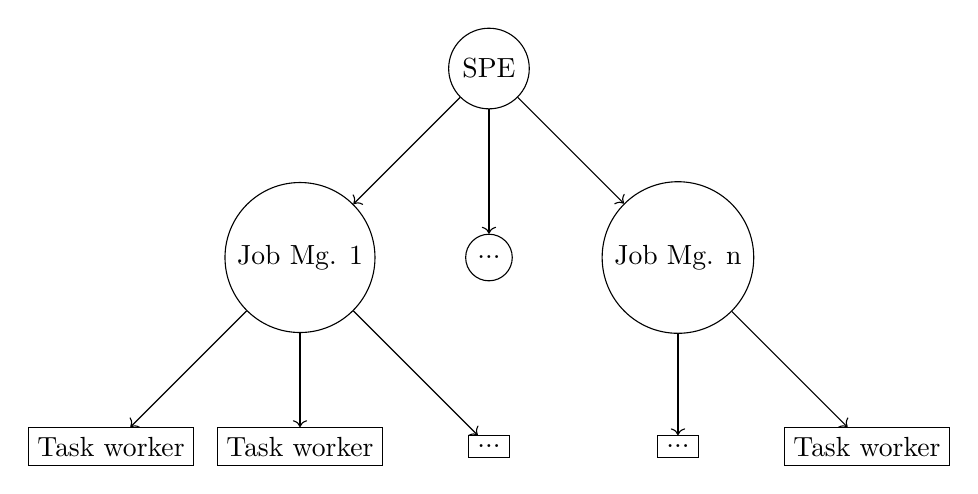
\begin{tikzpicture}[node distance=2.4cm, auto]
  \node[draw, circle] (SPE) {SPE};
  \node[draw, circle, below of=SPE] (JM2) {...};
  \node[draw, circle, left of=JM2] (JM1) {Job Mg. 1};
  \node[draw, circle, right of=JM2] (JM3) {Job Mg. n};
  
  \node[draw, rectangle, below of=JM1] (TW11) {Task worker};
  \node[draw, rectangle, right of=TW11] (TW12) {...};
  \node[draw, rectangle, right of=TW12] (TW13) {...};
  \node[draw, rectangle, left of=TW11] (TW14) {Task worker};

  \node[draw, rectangle, right of=TW13] (TWn) {Task worker};
  
  \draw[->] (SPE) to (JM1) ;
  \draw[->] (SPE) to (JM2) ;
  \draw[->] (SPE) to (JM3) ;

  \draw[->] (JM1) to (TW11) ;
  \draw[->] (JM1) to (TW12) ;
  \draw[->] (JM3) to (TW13) ;
  \draw[->] (JM1) to (TW14) ;

  \draw[->] (JM3) to (TWn) ;

\end{tikzpicture}
\end{center}
\end{figure}
\end{frame}

\begin{frame}{Messages}
    \begin{table}[]
        \centering
        \begin{tabular}{|c|c|}
        \hline
        TO: & Message \\
        \hline
        \hline
        Job manager &  \\
        Task worker & Handle cast \\
        \hline
        \end{tabular}
        \caption{SPE table}
    \end{table}

    \begin{table}[]
        \centering
        \begin{tabular}{|c|c|}
        \hline
        TO: & Message \\
        \hline
        \hline
        Job manager &  \\
        Task worker & Handle cast \\
        \hline
        \end{tabular}
        \caption{Job manager}
    \end{table}
    \begin{table}[]
        \centering
        \begin{tabular}{|c|c|}
        \hline
        TO: & Message \\
        \hline
        \hline
        Job manager &  \\
        Task worker & Handle cast \\
        \hline
        \end{tabular}
        \caption{SPE table}
    \end{table}
\end{frame}

\begin{frame}{SPE}
    \begin{table}[]
        \centering
        \begin{tabular}{|c|c|}
        \hline
        TO: & Message \\
        \hline
        \hline
        Job manager &  \\
        Task worker & Handle cast \\
        \hline
        \end{tabular}
        \caption{Task worker}
    \end{table}
\end{frame}

\end{document}